% Źródła: materialy/2026-10-12/wlasnosci-zeszyt.png i IMG_6916.jpeg.
% Numeracja 6, 7 według tablicy; podaddytywność w punkcie 5.
\section{Własności prawdopodobieństwa}
\label{sec:wlasnosci}

\begin{twierdzenie}
\label{tw:wlasnosci}
Niech $(\Omega,\F,\PP)$ będzie przestrzenią probabilistyczną.
Wówczas zachodzą następujące własności.
\begin{enumerate}[label=\arabic*),ref=\arabic*]
  \item\label{wlasn:zakres}
    Dla każdego $A\in\F$ zachodzi
    \[
      0\leq\PP(A)\leq1.
    \]
  \item\label{wlasn:pewne}
    Zdarzenie niemożliwe i zdarzenie pewne mają prawdopodobieństwa
    \[
      \PP(\varnothing)=0,\qquad \PP(\Omega)=1.
    \]
  \item\label{wlasn:dopelnienie}
    Dla każdego $A\in\F$ zachodzi
    \[
      \PP(A^c)=1-\PP(A).
    \]
  \item\label{wlasn:monotonicznosc}
    Jeżeli $A,B\in\F$ oraz $A\subseteq B$, to
    \[
      \PP(A)\leq\PP(B).
    \]
  \item\label{wlasn:suma}
    Dla $A,B\in\F$ mamy
    \[
      \PP(A\cup B)=\PP(A)+\PP(B)-\PP(A\cap B)
        \leq\PP(A)+\PP(B).
    \]
    Ogólniej, dla dowolnych zdarzeń $A_1,A_2,\ldots\in\F$
    zachodzi \emph{przeliczalna podaddytywność}:
    \[
      \PP\!\left(\bigcup_{n=1}^{\infty}A_n\right)
        \leq\sum_{n=1}^{\infty}\PP(A_n).
    \]
  \item\label{wlasn:rosnacy}
    Jeżeli $A_1\subseteq A_2\subseteq\cdots$ jest rosnącym
    ciągiem zdarzeń, to
    \begin{equation}
      \PP\!\left(\bigcup_{n=1}^{\infty}A_n\right)
        =\lim_{n\to\infty}\PP(A_n).
      \label{eq:ciag-rosnacy}
    \end{equation}
  \item\label{wlasn:malejacy}
    Jeżeli $A_1\supseteq A_2\supseteq\cdots$ jest malejącym
    ciągiem zdarzeń, to
    \begin{equation}
      \PP\!\left(\bigcap_{n=1}^{\infty}A_n\right)
        =\lim_{n\to\infty}\PP(A_n).
      \label{eq:ciag-malejacy}
    \end{equation}
\end{enumerate}
\end{twierdzenie}

% Wszystkie stwierdzenia powyżej należą do wykładu 1.
% Według polecenia użytkownika wykład 2 zaczyna się od dowodu 6.
\poczatekwykladu{2}

\begin{proof}[Dowód własności \ref{wlasn:rosnacy}]
Przyjmijmy $A_0=\varnothing$ i zdefiniujmy
\[
  B_n=A_n\setminus A_{n-1},\qquad n=1,2,\ldots.
\]
Zdarzenia $B_n$ są parami rozłączne; ilustruje to
rysunek~\ref{fig:ciag-rosnacy}. Ponadto dla każdego $N\geq1$
\[
  \bigcup_{n=1}^{N}B_n=\bigcup_{n=1}^{N}A_n=A_N,
  \qquad
  \bigcup_{n=1}^{\infty}B_n=\bigcup_{n=1}^{\infty}A_n.
\]
Z przeliczalnej addytywności otrzymujemy
\begin{align*}
  \PP\!\left(\bigcup_{n=1}^{\infty}A_n\right)
    &=\PP\!\left(\bigcup_{n=1}^{\infty}B_n\right)
      =\sum_{n=1}^{\infty}\PP(B_n)\\
    &=\lim_{N\to\infty}\sum_{n=1}^{N}\PP(B_n)
      =\lim_{N\to\infty}\PP\!\left(\bigcup_{n=1}^{N}B_n\right)\\
    &=\lim_{N\to\infty}\PP(A_N).
\end{align*}
\end{proof}

\begin{figure}[H]
  \centering
  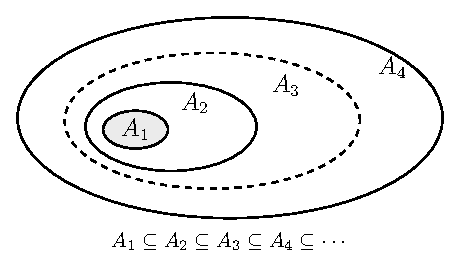
\includegraphics[width=8.2cm]{ciag-zdarzen-rosnacy.pdf}
  \caption{Rosnący ciąg zdarzeń. Kolejne różnice
    $B_n=A_n\setminus A_{n-1}$ są parami rozłączne.}
  \label{fig:ciag-rosnacy}
\end{figure}

\begin{proof}[Dowód własności \ref{wlasn:malejacy}]
Skoro $A_1\supseteq A_2\supseteq\cdots$, to
$A_1^c\subseteq A_2^c\subseteq\cdots$. Korzystamy z prawa
de Morgana oraz z udowodnionej własności \ref{wlasn:rosnacy}:
\begin{align*}
  \PP\!\left(\bigcap_{n=1}^{\infty}A_n\right)
    &=1-\PP\!\left(\left(\bigcap_{n=1}^{\infty}A_n\right)^c\right)\\
    &=1-\PP\!\left(\bigcup_{n=1}^{\infty}A_n^c\right)\\
    &=1-\lim_{n\to\infty}\PP(A_n^c)
      =\lim_{n\to\infty}\bigl(1-\PP(A_n^c)\bigr)\\
    &=\lim_{n\to\infty}\PP(A_n).
\end{align*}
\end{proof}
